\subsection{FreeTSA i timestamping}
\label{arquitectura:timestamping}
%Entrant més a baix nivell, d'acord amb l'standard definit a l'RFC3161\footnote{https://tools.ietf.org/html/rfc3161} el que s'anomena \textit{trusted timestamp} és un \textit{timestamp} emès per una  TSA\footnote{\textbf{T}ime \textbf{S}tamp \textbf{A}uthority} que es fa servir per a provar l'existència d'un cert contingut en un moment determinat.\\
%\newline A la figura següent (Figura \ref{fig:trusted_timestamping}) es pot veure el funcionament del procés de segellat de temps:
%\begin{figure}[h]
%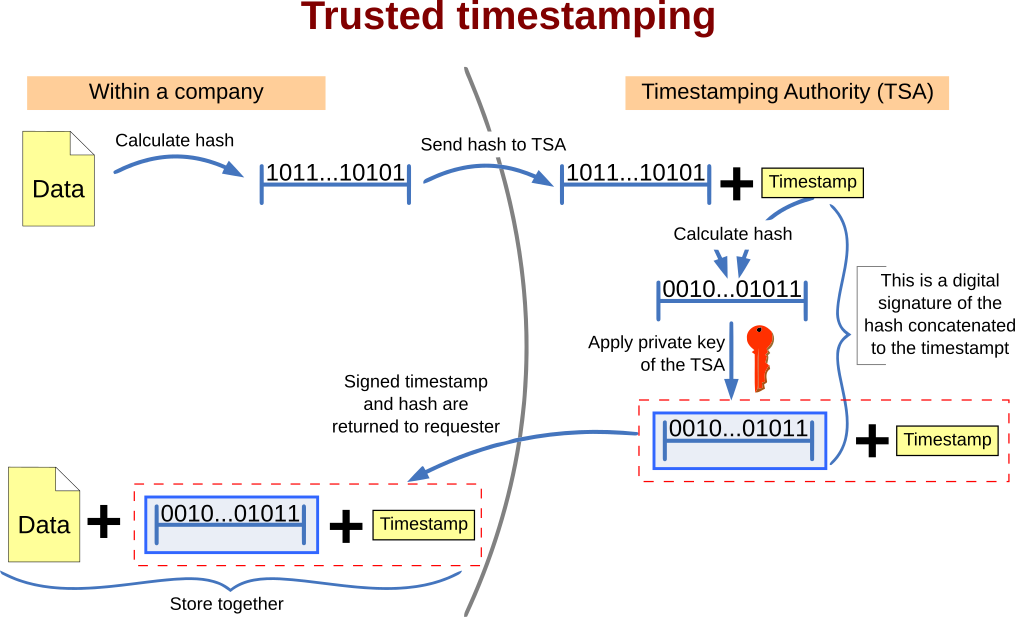
\includegraphics[scale=0.5]{sections/arquitectura/trusted_timestamping.png}
%\centering
%\caption{Generació i certificació de documents}
%\label{fig:trusted_timestamping}
%\end{figure}
%\newline A la figura anterior, es pot apreciar el funcionament del servei de segellat de temps de FreeTSA\footnote{https://freetsa.org/index_en.php} (entitat certificadora que es fa servir pel projecte).
%\newline En el cas concret del projecte, l'entitat que juga el rol de \textit{TSA}, és \textit{FreeTSA}\footnote{https://freetsa.org/index_en.php}.\\
%Com la gran majoria de serveis, ofereix una API (en aquest cas oberta) per a que els desenvolupadors puguin fer ús de les funcionalitats implementades.\\
%El funcionament del servei és ben senzill, primerament s'ha de generar un fitxer .tsq (\textit{time stamp query}) amb el contingut sobre el qual volem realitzar el segellat de temps. Aqesut fitxer, l'enviarem via HTTP/Post al servei de FreeTSA que respondrà amb un fitxer .tsr (\textit{time stamp request}).\\
%\newline Aquest fitxer .tsq, juntament amb els fitxers .pem i .tsc (donats pel mateix servei) ens serviràn posteriorment per validar el \textit{hash} dels documents.\\ És de vital importància el desar aquest fitxer .tsc, ja que és clau en el cas de necessitar defensar la integritat del comprovant de signatura mitjançant el segellat de temps.

Alternativament a l'ús de \textit{blockchain}, com a mesura de certificació addicional i per a donar més confiança, s'ha optat per donar al sistema un tercer cas d'ús.\\
\newline Tornant a la Figura \ref{fig:hash_timestamping_usecase}, al llarg d'aquesta secció es parlarà sobre el tercer i últim cas d'us, anomenat ``segellat de temps amb el hash''.\\
\newline Per aquest cas d'ús, es busca donar la confiança suficient a aquells que no vegin amb bons ulls l'ús de \textit{blockchain} com a mètode per a certificar l'existència d'un document en un instant de temps determinat.\\
Alhora, com s'ha dot anteriorment, suposa un extra que sempre és benvingut.\\
\newline Per aquesta ocasió, l'estructura i funcionament és molt similar al que s'ha vist la secció vista anteriorment (\ref{arquitectura:blockchain}). Dos serveis, un pertanyent a l'aplicació, amb l'objectiu d'encapsular i donar accés, i l'altre, un servei extern de tercers que ofereix funcions de segellat de temps.
\newline L'ús de serveis externs obliga a l'ús d'adaptadors que facin la funció d'enllaç entre l'aplicació desenvolupada per aquest projecte, i el servei extern.
% que ens permet realitzar el segellat de temps sobre el contingut d'un fitxer. Per a realitzar el segellat de temps, farem servir el \textit{hash} sobre el contingut d'aquest fitxer.

